% % % % % % % % % % % % % % % % % % % % % % % % % % % % % % % % % %
%  Devolutiva — Fase 1: Imersão
%  Disciplina: Design Thinking (DE_233) — ETE Cícero Dias
%  Profa. Samara Silva  ·  Recife, 19 de junho de 2026
% % % % % % % % % % % % % % % % % % % % % % % % % % % % % % % % % %

\documentclass[
  sigconf,
  nonacm, % Remove o rodapé da ACM
  language=portuguese
]{acmart}

% ── Desliga rodapé ACM ──────────────────────────────────────
\settopmatter{printacmref=false}
\setcopyright{none}
\acmYear{2026}
\let\balance\relax

% ── Mata a página temporária da ACM (compilação única via API) ──
\makeatletter
\def\acm@addtemp@page{}
\makeatother

% ── Pacotes ─────────────────────────────────────────────────
\usepackage[portuguese]{babel}
\usepackage{microtype}
\usepackage{booktabs}
\usepackage{tabularx}
\usepackage{array}
\usepackage{colortbl}
\usepackage[dvipsnames,table]{xcolor}
\usepackage[inline]{enumitem}
\usepackage{graphicx}
\usepackage{adjustbox}
\usepackage{fancyhdr}
\usepackage{eso-pic} % Para a capa preencher toda a página sem gerar páginas em branco

% ── Ajuste contra quebras de texto ruins (Textos Cortados) ──
\tolerance=1000
\emergencystretch=1.5em

% ── Cores ───────────────────────────────────────────────────
\definecolor{cgood}{HTML}{1E6B3A}
\definecolor{cwarn}{HTML}{8B4500}
\definecolor{cred}{HTML}{C0392B}
\definecolor{cmuted}{HTML}{666666}
\definecolor{crow}{HTML}{F2EFEB}

% ── Colunas customizadas para tabela ────────────────────────
\newcolumntype{L}[1]{>{\raggedright\arraybackslash}p{#1}}
\newcolumntype{C}[1]{>{\centering\arraybackslash}p{#1}}

% ── Comando nota destacada ───────────────────────────────────
\newcommand{\notadestaque}[2]{%
  \noindent\textbf{Nota:}\enspace%
  {\large\bfseries\color{cred}#1\,/\,#2\,pts}%
}

% ── Comando label de status ──────────────────────────────────
\newcommand{\statusok}[1]{{\small\bfseries\color{cgood}#1}}
\newcommand{\statuswarn}[1]{{\small\bfseries\color{cwarn}#1}}

% ── Renomeações PT-BR ────────────────────────────────────────
\AtBeginDocument{%
  \renewcommand{\abstractname}{Resumo}
  \renewcommand{\figurename}{Figura}
  \renewcommand{\tablename}{Tabela}
}

% ────────────────────────────────────────────────────────────
\begin{document}

% ── CAPA ────────────────────────────────────────────────────
\thispagestyle{empty}
\AddToShipoutPictureBG*{%
  \AtPageLowerLeft{%
    \IfFileExists{capa.png}{%
      
\includegraphics[width=\paperwidth,height=\paperheight]{capa.png}%
    }{%
      \IfFileExists{../../capa.png}{%
        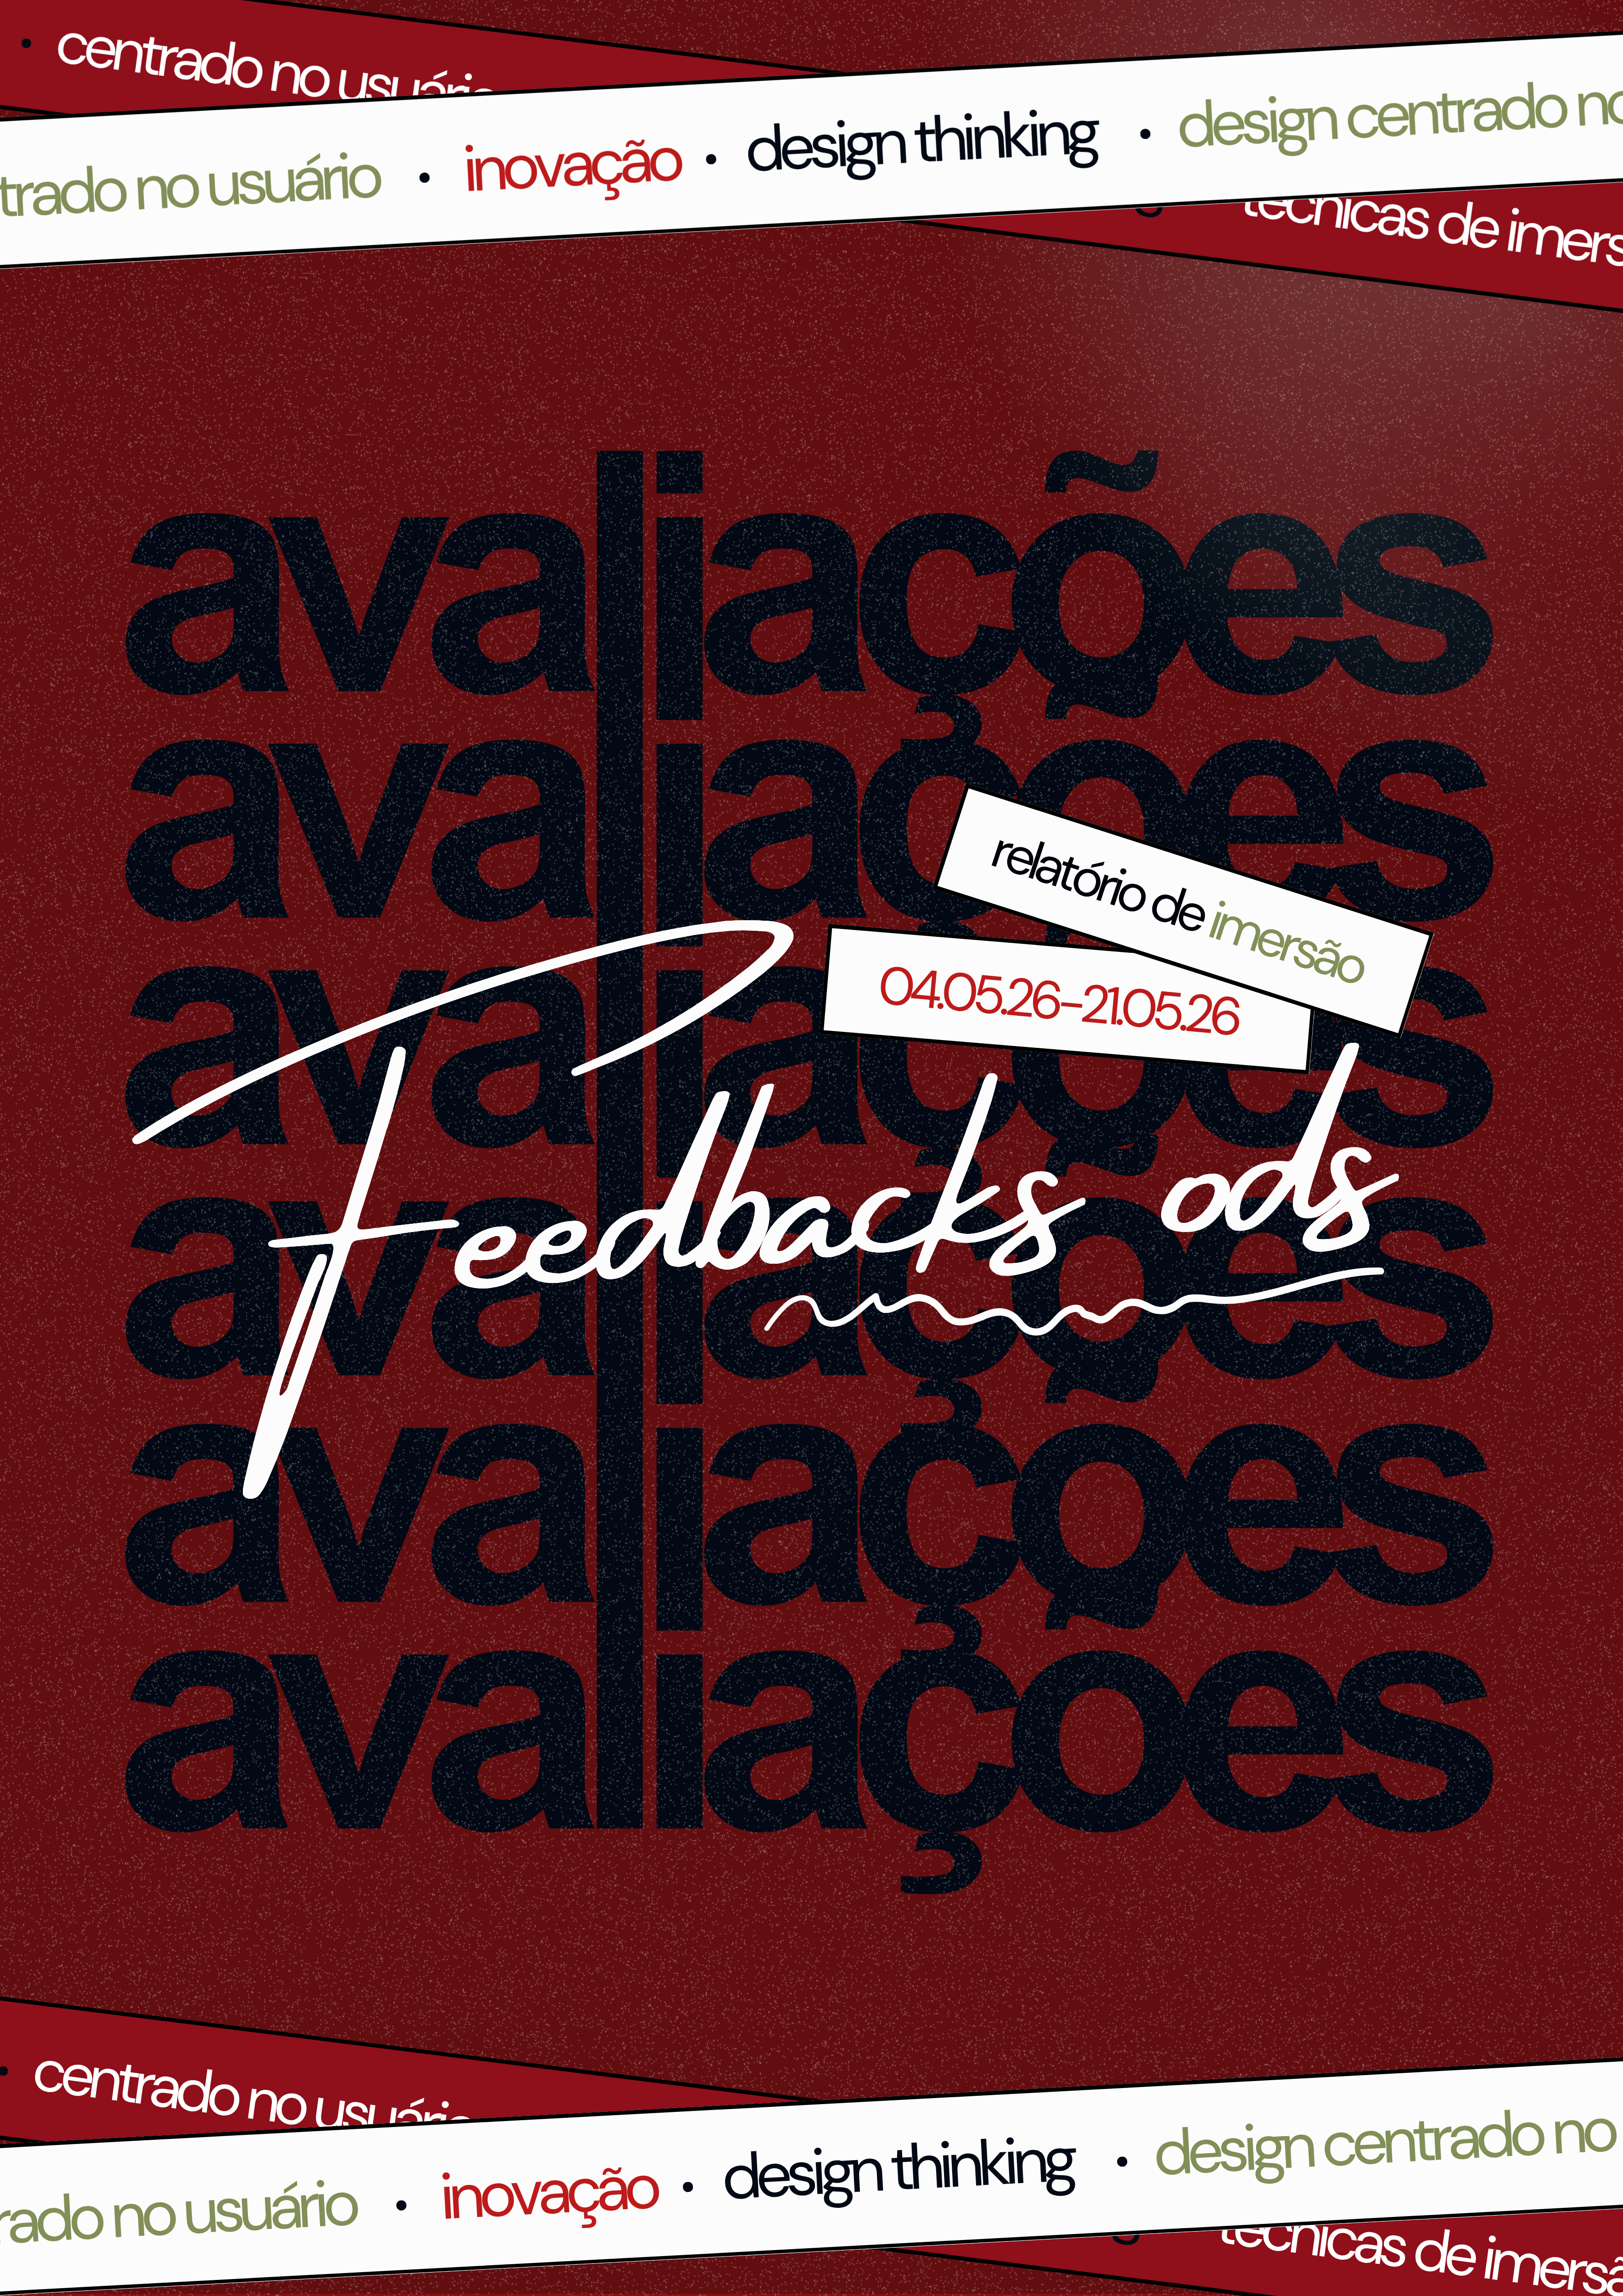
\includegraphics[width=\paperwidth,height=\paperheight]{../../capa.png}%
      }{%
        \parbox[b][\paperheight]{\paperwidth}{%
          \vspace*{10cm}\begin{center}{\large\color{gray}[capa.png não encontrada]}\end{center}%
        }%
      }%
    }%
  }%
}
\mbox{} % Caixa vazia para garantir que a página da capa seja gerada e preenchida
\clearpage

% ── CONFIGURAÇÃO DE PÁGINA PÓS-CAPA ─────────────────────────
\setcounter{page}{1}
\pagestyle{fancy}
\fancyhf{}
\renewcommand{\headrulewidth}{0pt}
\fancyfoot[C]{\thepage}
\setlength{\headsep}{0.8cm} % Distancia o cabeçalho do conteúdo das colunas

% ── METADADOS ────────────────────────────────────────────────
\title{Feedback Avaliativo de Projeto: Projeto Integrador I --- Relatório de Definição}

\author{Profa.\ Samara Silva}
\authornote{Grupo: \textbf{Grupo 01 - Fome Zero} \textperiodcentered\ Per\'{i}odo: 22 de maio de 2026 \textperiodcentered\ Avaliado em: 19 de junho de 2026.}
\email{samarasilvia.educa@gmail.com}
\affiliation{%
  \institution{ETE C\'{i}cero Dias}
  \department{M\'{o}dulo 1 --- Turma A · 2026.1}
  \city{Recife}
  \state{Pernambuco}
  \country{Brasil}
}

\author{Grupo 01 - Fome Zero}
\affiliation{%
  \institution{ETE C\'{i}cero Dias}
  \department{Turma --- Turma A · 2026.1}
  \city{Recife}
  \state{Pernambuco}
  \country{Brasil}
}
\maketitle

\vspace{1em}
\section{Avaliação Geral}

\notadestaque{0,70}{1,00}

A avaliação foi concluída. A seguir o resumo dos critérios e os comentários detalhados.

\subsection{Resumo dos Critérios}

\rowcolors{2}{crow}{white}
\begin{tabular}{@{} L{2.6cm} C{2.5cm} C{1.1cm} C{1.1cm} @{}}
\toprule
\textbf{Critério} & \textbf{Status} & \textbf{Nota} & \textbf{Máx.} \\
\midrule
Relatório de Definição & \statuswarn{Completo, mas inadequado} & \textbf{0,70} & 1,00 \\
\midrule
\textbf{Total} & & \textbf{\color{cred}0,70} & \textbf{1,00} \\
\bottomrule
\end{tabular}

\section{Comentários por Critério}

\subsection{Relatório de Definição}

\noindent\statuswarn{0,70\,/\,1,00 pts · Completo, mas inadequado}

\begin{itemize}[leftmargin=14pt,itemsep=1pt,topsep=3pt,parsep=0pt]
  \item[\textcolor{cgood}{$\checkmark$}] {\small\textcolor{cgood}{Há coerência entre o que foi descoberto na Imersão e o que foi definido como problemática}}
  \item[\textcolor{cgood}{$\checkmark$}] {\small\textcolor{cgood}{A narrativa do documento cresce de forma cumulativa}}
  \item[\textcolor{cgood}{$\checkmark$}] {\small\textcolor{cgood}{A seção de Definição está integrada ao documento — não é um arquivo solto}}
  \item[\textcolor{cgood}{$\checkmark$}] {\small\textcolor{cgood}{Os artefatos de prsona, mapa de empatia, jornada e enunciado do problema estão documentados com clareza}}
  \item[$\square$] {\small\textcolor{cmuted}{A descrição textual da persona está complementando o artefato (img) construída}}
  \item[$\square$] {\small\textcolor{cmuted}{Na descrição textual da persona foi justificado a escolha da quantidade de personas}}
  \item[$\square$] {\small\textcolor{cmuted}{Na descrição textual da persona foi justificado o público alvo priorizado ao qual foi baseada}}
  \item[\textcolor{cgood}{$\checkmark$}] {\small\textcolor{cgood}{Na seção de referências está inserido o link do figma dos artefatos de definição}}
\end{itemize}

O relatório, embora muito bem escrito e estruturado nesta fase de definição, apresenta uma limitação importante no que se refere à complementação dos artefatos visuais (imagens). Observa-se que, de forma geral, as descrições textuais se restringem à transcrição direta do conteúdo presente nos artefatos, sem uma ampliação interpretativa ou analítica das informações apresentadas.

Dessa forma, o texto acaba não explorando o potencial reflexivo esperado nesta etapa, que seria justamente a capacidade de interpretar os dados dos artefatos, conectar informações relevantes e justificar as escolhas de design a partir desses elementos. A ausência dessa camada analítica reduz a profundidade do relatório, tornando-o mais descritivo do que investigativo.

\textit{\textbf{Feedback relacionado ao dt E dcu}}

De forma geral, os artefatos demonstram boa execução dentro da lógica de Design Thinking, especialmente no que se refere à organização, estrutura e apresentação visual das informações. No entanto, sob a perspectiva do Design Centrado no Usuário, ainda existem lacunas relacionadas à profundidade da análise da experiência do usuário.

Essas lacunas envolvem principalmente a ausência de elementos como comportamento digital, contexto real de uso, limitações situacionais, canais utilizados e fricções na interação. O aprofundamento desses aspectos contribuiria para uma compreensão mais completa do usuário e, consequentemente, para decisões de design mais consistentes e fundamentadas.

\textit{\textbf{Feedback relacionado a persona}}

No relatório é mencionada a construção de uma segunda persona, porém não fica claro qual foi a primeira. Além disso, a descrição apresentada não deve ser apenas uma repetição do que foi feito no Figma, mas sim uma versão mais analítica e descritiva da persona, trazendo interpretações, contexto e aprofundamento.

Também não foram apresentadas justificativas adequadas para a construção da persona. O conteúdo parece, em grande parte, uma transcrição direta dos artefatos feitos no figma, sem uma análise crítica ou explicação sobre quais informações foram priorizadas a partir da etapa de imersão.

Um relatório mais consistente deveria evidenciar, por exemplo, quais dados foram mais recorrentes nas pesquisas, como eles influenciaram na construção da persona e quais decisões foram tomadas a partir disso. No exemplo trabalhado em sala com Adalberto, há uma contextualização inicial baseada em dados predominantes, como sua atuação no comércio local e a dependência econômica do mercadinho, além da justificativa clara das escolhas feitas na construção do perfil.

Por fim, também não foi apresentada uma justificativa para a escolha de apenas uma persona, o que seria importante para dar coerência metodológica ao trabalho.

\textit{\textbf{Feedback relacionado ao mapa de empatia e jornada do usuário}}

Durante a criação do template da segunda fase do Design Thinking, foram incluídos inicialmente outros artefatos, como o POV, além de uma descrição mais detalhada do mapa de empatia e da jornada do usuário. Em sala, foi reforçado que esses elementos não seriam mais obrigatórios nessa etapa.

Nesse sentido, é louvável e interessante que o grupo tenha mantido esses artefatos no material, demonstrando cuidado e aprofundamento na entrega. No entanto, assim como observado na persona, tanto o mapa de empatia quanto a jornada do usuário acabam se apresentando como uma transcrição direta dos dados presentes nos artefatos visuais (imagens), sem uma análise mais interpretativa ou reflexão sobre as informações levantadas.

Seria importante que esses elementos não se limitassem à reprodução do conteúdo dos quadros, mas sim que trouxessem uma camada de análise, conectando os dados coletados com insights relevantes para o projeto. Isso incluiria, por exemplo, a identificação de padrões de comportamento, dores mais recorrentes e oportunidades de solução derivadas da interpretação dos dados.

Dessa forma, os artefatos deixariam de ser apenas descritivos e passariam a cumprir um papel mais analítico dentro do processo de design thinking, contribuindo de forma mais consistente para a etapa de definição do problema e construção da solução.

\section{Considerações Finais}

Os ajustes indicados são de natureza metodológica e devem ser
incorporados para as próximas entregas.
Continuem assim.

% ── Assinatura ───────────────────────────────────────────────

\vspace{1.5em}
\noindent\rule{\linewidth}{0.4pt}

\begin{flushright}
\textbf{Profa.\ Samara Silva}\\
{\small\color{cmuted} Design Thinking --- DE\_233 · ETE Cícero Dias}\\
{\small\color{cmuted} Recife, 19 de junho de 2026}
\end{flushright}

% ── Sem referências bibliográficas ───────────────────────────

\appendix
\onecolumn
\section{Critérios e Níveis de Avaliação}

Esta seção apresenta os critérios de avaliação para referência dos estudantes.

\subsection{Níveis de Completude}

\begin{tabularx}{\linewidth}{@{} p{4cm} p{1.5cm} X @{}}
\toprule
\textbf{Nível} & \textbf{\%} & \textbf{Descrição} \\
\midrule
Completo & 100\% & Fez tudo e fez certo. Critério plenamente atendido. \\
Completo c/ ressalvas & 85\% & Fez tudo, mas algo ficou incorreto ou impreciso. Esforço total, qualidade com falha. \\
Completo, mas inadequado & 70\% & Preencheu todos os itens, porém boa parte do conteúdo não atende ao propósito da atividade. \\
Faltou pouco & 65\% & Fez bastante e acertou o que fez. Faltaram partes, mas o que entregou presta. \\
Faltou pouco c/ erros & 60\% & Fez bastante, mas errou partes relevantes. Metade do caminho com qualidade irregular. \\
Faltou muito & 40\% & Fez pouco, mas o que fez está correto. Entrega incompleta, execução ok. \\
Faltou muito e errou & 25\% & Fez pouco e ainda errou. Esforço baixo, qualidade baixa. \\
Errado & 10\% & Tentou, mas a abordagem foi incorreta por completo. Reconhece a tentativa. \\
Não fez & 0\% & Critério não entregue. \\
\bottomrule
\end{tabularx}

\vspace{1em}
\subsection{Penalizações por Atraso}

\begin{tabularx}{0.6\linewidth}{@{} X p{5cm} @{}}
\toprule
\textbf{Atraso} & \textbf{Desconto} \\
\midrule
Até 1 dia & -10\% \\
2–3 dias & -20\% \\
Mais de 3 dias & -30\% \\
Não entregou & Zera a nota \\
\bottomrule
\end{tabularx}

\section{Devolutiva Individual}

A nota individual é calculada aplicando o fator de contribuição sobre a nota do grupo em cada fase.

\subsection{Fatores de Contribuição}

\begin{tabularx}{0.6\linewidth}{@{} X c @{}}
\toprule
\textbf{Fator} & \textbf{Multiplicador} \\
\midrule
Liderou & 100\% \\
Participou & 100\% \\
Participou pouco & 70\% \\
Só fez sua parte & 40\% \\
Não participou & 0\% \\
\bottomrule
\end{tabularx}

\vspace{1em}
\subsection{Notas por Integrante}

\begin{tabularx}{\linewidth}{@{} X X p{2.5cm} @{}}
\toprule
\textbf{Integrante} & \textbf{\small PI Relatório de Definição} & \textbf{Total} \\
\midrule
André da Silva Durães & \textit{---} & \textbf{0,00} \\
Bruna Maria do Nascimento Costa & \textit{---} & \textbf{0,00} \\
João Gabriel Cavalcanti & 0,70 \textit{(Participou)} & \textbf{0,70} \\
Suammyr Cavalcante do Carmo & 0,70 \textit{(Participou)} & \textbf{0,70} \\
Maria Zilda Ferreira Pinto & 0,70 \textit{(Participou)} & \textbf{0,70} \\
Ayran Gabriel Duque Souza Lima & \textit{---} & \textbf{0,00} \\
\bottomrule
\end{tabularx}

\end{document}
